\documentclass[11pt]{article}
\usepackage[margin=1in]{geometry}
\usepackage{amsmath, amssymb, amsthm, enumerate}
\usepackage{graphicx,url, hyperref,framed, esint, color, tikz}

\setcounter{secnumdepth}{-2}

\begin{document}
\begin{flushright}
Alex Rich and Aaron Rosen\\
Engineering 155 \\ 
Final Project Proposal\\
November 16, 2015
\end{flushright}
\section{Project Status Report: A Robot Controlled Over The Internet}

***\\
Report should include:\\
A 4-page report (plus appendices) documenting your design at the midpoint. The status should include 
%\\- schematics of anything on a breadboard, 
\\- block diagrams of the logic on your FPGA, 
%\\- and an outline of the routines used on the Pi. 
\\ You should include as an appendix either your Verilog code or software that is mostly complete (but do not have to have both ready). 
\\- You must be ready to demonstrate some working hardware in the lab.
\\***

The team has made progress on a robotic vehicle that receives user input from a website and executes them. The website is hosted by an E155 Raspberry Pi2 Apache2 server, and contains a visual grid interface.  The user  clicks on different points on the grid to input commands into a buffer to be sent to the vehicle.  The Pi will parse the commands and send them using a Belkin FT8001 bluetooth dongle to a BlueSMiRF on the vehicle.  The vehicle�s controller (the E155 $\mu$Mudd board) reads these commands and executes them. An overview of this system is shown in Figure \ref{fig:sys}. Below we discuss the current status for each part (website, Pi, FPGA, vehicle, new hardware) in detail.

\subsection{Website}
The website contains a visual user interface that contains instructions for use, a grid on which to input locations for the robot to maneuver to, a list of the locations currently buffered for sending, a �clear buffer.� The code for the website is shown in Appendix A. The website was built using HTML, Javascript, and Bootstrap CSS. 

\subsection{Raspberry Pi 2}
The Pi hosts the website. Upon clicking in a grid space, the page's javascript calculates the left and right tread speeds and duration of movement required to get the tank to move from its original position to the new position. Next, the javascript makes an HTTP GET request to the inputChars resource of the Pi. When the request is completed, the page updates, either submitting the next command in the buffer or waiting for another input from the user.

After receiving a GET request, the common gateway interface (CGI) reads the input parameters and calls a Python script. The Python script utilizes the \verb.bluetooth. module to allow sending data using the bluetooth dongle. Since the robot has a constant bluetooth device address, this address is hard coded into the Python script. When called, the python script sends the commands, one at a time, to the robot. Currently, the system sleeps for an amount of time to theoretically give the tank enough time to move, however in the future, the Pi should wait for acknowledgement from the FPGA. The code on the Pi is shown in Appendix B. In summary, here is the order in which the Pi responds to user input.

\subsection{FPGA}
The FPGA reads data from a BlueSMiRF using UART communication.  The UART is implemented using a PLL clock.  The FPGA will execute the command received by controlling the two motors via the H-Bridges on the $\mu$Mudd board. The SystemVerilog code running on the FPGA is sown in Appendix C. The FPGA and BlueSMiRF are the only two electrical components on the breadboard. The schematic is shown in figure \ref{fig:breadboard}


\begin{figure}
\begin{center}
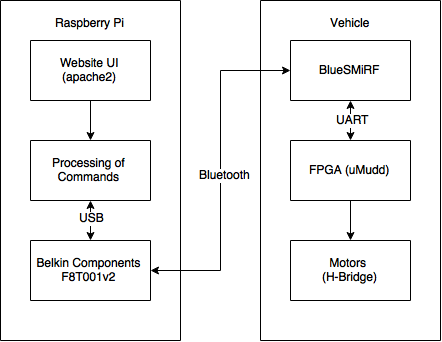
\includegraphics[width=0.7\textwidth]{E155System}
\end{center}
\caption{An overview of the system. The system is comprised of two major subsystems: the Raspberry Pi 2 controller and the vehicle, which is controlled by the $\mu$Mudd board.}
\label{fig:sys}
\end{figure}

\subsection{Vehicle}
The mechanics of the vehicle have not been constructed yet, since this will largely be snapping pieces together.

\begin{figure}
\begin{center}
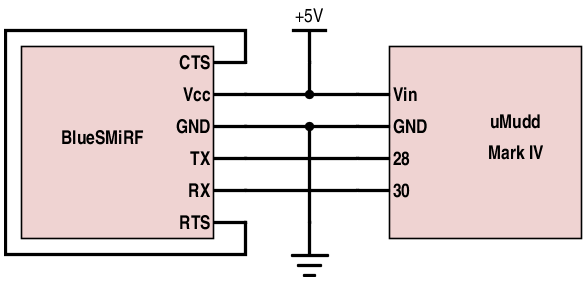
\includegraphics{breadboard}
\end{center}
\caption{The schematic of the circuit on the breadboard. In simple applications, the CTS and RTS pins of the BlueSMiRF are connected together, and the only pins that are connected to the FPGA are TX and RX.}
\label{fig:breadboard}
\end{figure}



\section{Appendix A: Website}
\subsection{Code}

\subsection{Result}

\section{Appendix B: Raspberry Pi2 Code}
\section{Appendix C: SystemVerilog Code on FPGA}

%
%\section{Bill of Materials}
%
%\centering
%\begin{tabular}{|l|l|l|l|}
%\hline
%\multicolumn{1}{|c|}{\textbf{Item}} & \multicolumn{1}{c|}{\textbf{Description}}               	& \multicolumn{1}{c|}{\textbf{Source}} & \multicolumn{1}{c|}{\textbf{Cost}} \\ \hline
%Tracked Vehicle 			&										&							&	\\
%			Chassis Kit	& Chassis for the tank, includes treads and frame.    	& Amazon 					& 15.39                          	\\ \hline
%Tamiya 70168				& Gives tank flexibility to turn by controlling each     	& 							& \\
%Double Gearbox			& tread independently.						& Amazon		               			& 11.99                             	\\ \hline
%$\mu$Mudd Board                	& Controls the vehicle                                                 & E155                                 		& 0.00                               	\\ \hline
%			                      	& Provides website interface and sends commands 	&							&\\
%Raspberry Pi 2			    	& to vehicle             							& E155                                 		& 0.00                               	\\ \hline
%                        				& Wirelessly communicate via Bluetooth between  	&							&\\
%2X BlueSMiRF				& Pi and $\mu$Mudd board. 					& E155                                		& 0.00                               	\\ \hline
%2X TrustFire 14500			& Li Ion battery, 3.7 V 						& Aaron Rosen					& 0.00				\\ \hline
%\end{tabular}

\end{document}


























